In this paragraph some use cases will be described. These use cases can be derived from the scenarios and the use case diagram.

\begin{figure}[H]
   \begin{center}
    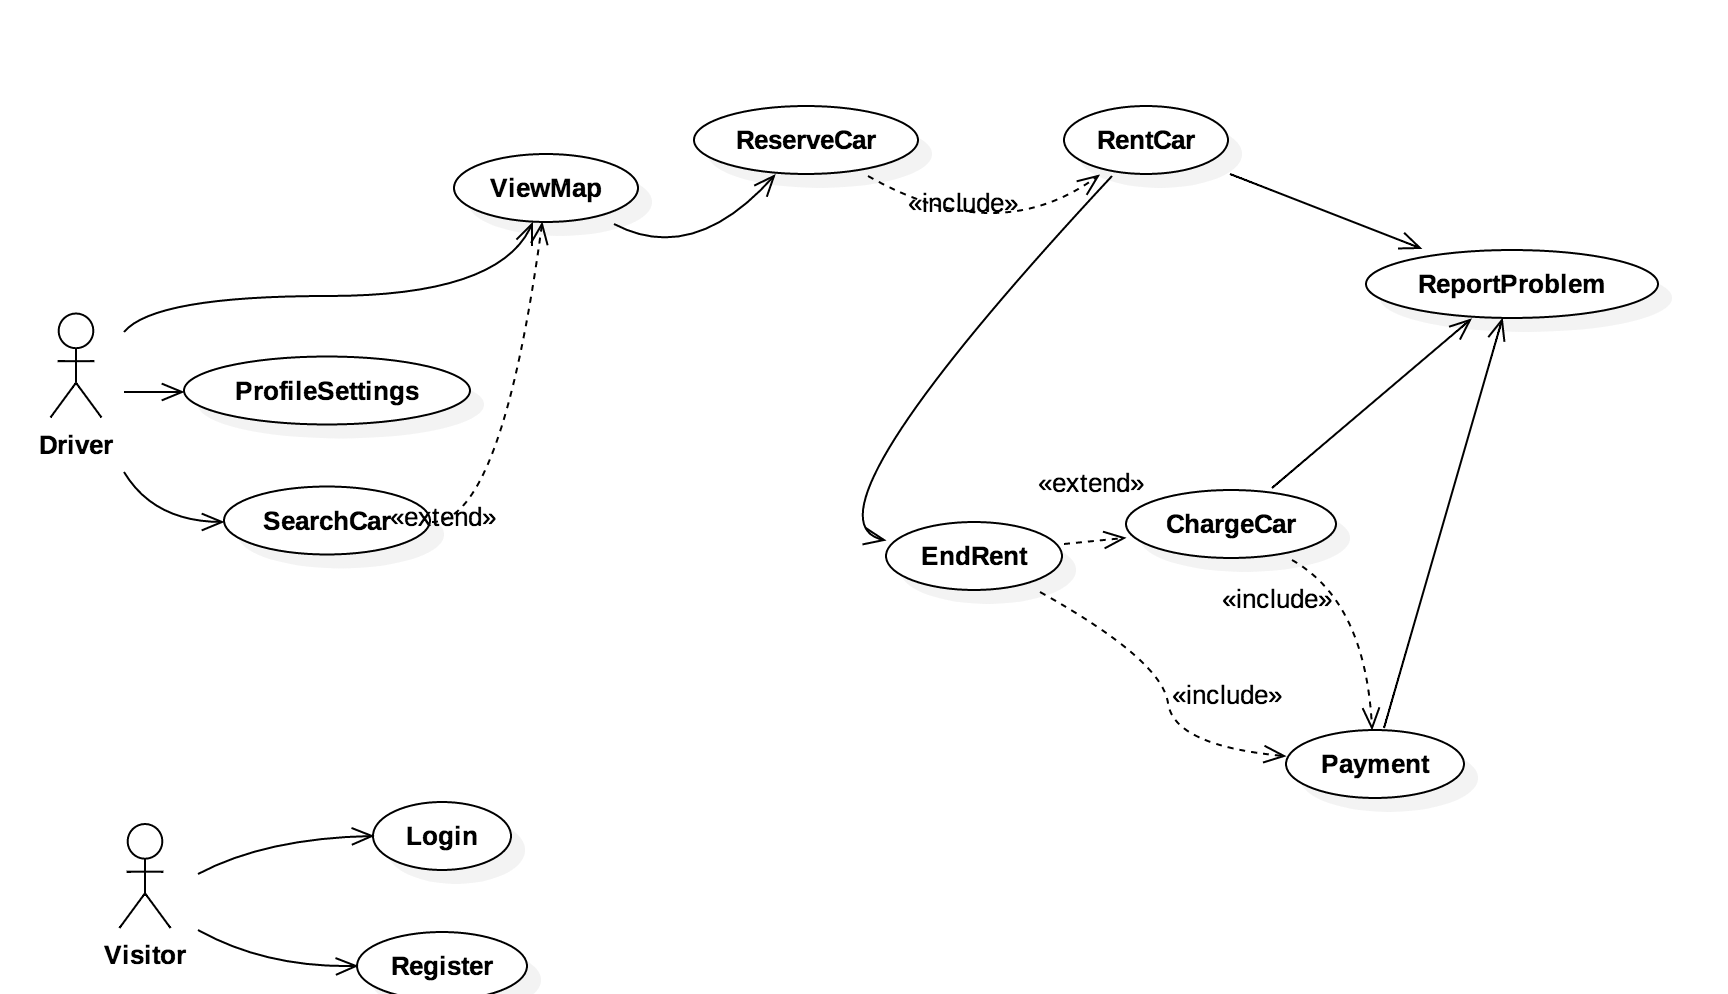
\includegraphics[width=\textwidth]{Resources/UseCaseModel.png}
    \caption{Use cases diagram}
   \end{center}
    \label{fig:UseCasesDiagram}
\end{figure}

\begin{center}
\line(1,0){250}
\end{center}

\begin{description}
	\item[Name:] User registration
	\item[Actors:] Visitor
	\item[Entry conditions:] There are no entry conditions
	\item[Flow of events:]  \ \\
		\begin{itemize}
			\item The visitor arrive to the home page of the application, as is not logged in is redirect to the login/registration page
			\item The visitor enter his personal information, his driver license, a photo of his driver license and some payment method
			\item The visitor clicks on the confirm button
			\item The application suggest the user to read his emails to receive the password
			\item The visitor login after read the password
		\end{itemize}
	\item[Exit conditions:] The visitor is redirect to the home page of the application
	\item [Exception:] The information furnished by the visitor are not correct or ambiguous as the following case:
		\begin{itemize}
			\item The Email has not the correct format
			\item The Birthday is not at least eighteen years ago
			\item The Payment method is not valid
			\item The information's of the driver license don't correspond with the information furnished by the visitor
			\item The Driver license is not valid
		\end {itemize}
		Also the visitor could had forgot to enter some requested camp or to accept the Terms and Conditions. In all this case, the system does not send any mail to the visitor but notifies him that an error has been made and allows to input the incorrect data again
	\end{description}
	
\begin{center}
\line(1,0){250}
\end{center}

\begin{description}
	\item[Name:] User Login
	\item[Actors:] User
	\item[Entry conditions:] There are no entry conditions
	\item[Flow of events:]  \ \\
		\begin{itemize}
			\item The user arrives at the Login page of the mobile application.
			\item The user inputs his email address and his password.
			\item The user clicks on the log in button.
			\item The system redirects the user to the home page.
		\end{itemize}
	\item[Exit conditions:] The user is successfully redirected to the application home page.
	\item [Exception:] The email and/or the password furnished by the user are not correct. In this case, the system does not redirect the user to the home page but notifies him that an error has been made and allows to input his email and password again. The user can also forget his/her password, in this case he/she can ask to generate another password and received it on his/her personal email address.
\end{description}

\begin{center}
\line(1,0){250}
\end{center}

\begin{description}
	\item[Name:] Reserve a car
	\item[Actors:] User, 
	\item[Entry conditions:] There is at least a car not reserved neither used.
	\item[Flow of events:]  \ \\
		\begin{itemize}
			\item The user arrives at the home page of the application that shows the map with the markers of the cars.
			\item The user choose a car.
			\item The user clicks on the marker of the car chosen.
			\item The user clicks on the "Reserve" button
			\item The application shows to the user the time remained to start the engine and the position of both the actors.
			\item The user arrives next to the car.
			\item The user clicks on the button "Open the car"
			\item The car is opened by the system
			\item The user get into the car and start the engine.
		\end{itemize}
	\item[Exit conditions:] The user successfully start the engine of the car
	\item [Exception:] Two users reserve the same car in a really small difference of time, the system in this case will delete the reservation that is requested later.
\end{description}

\begin{center}
\line(1,0){250}
\end{center}

\begin{description}
	\item[Name:] End a rent
	\item[Actors:] User, Car 
	\item[Entry conditions:] The car is in the state In Use
	\item[Flow of events:]  \ \\
		\begin{itemize}
			\item The user stop the engine of the car and get out of the vehicle.
			\item The car check if all the doors are closed and there is no one into the it.
			\item The system close the car
			\item The system wait 5 minute
			\item The system send the request for payment to the external system
			\item The external system answer to the request
			\item The system notify the user about the end of the rent with a message on the app
		\end{itemize}
	\item[Exit conditions:] The user successfully end the rent
	\item [Exception:] 
		\begin{itemize}
			\item The car is not parked in predefined area, in this case the system will not allow the user to end rent and close the car. 
			\item The payment request failed, in this case the system block the user and he/her will not be able to use the system  again until he complete the payment
			\item The car is stopped but the user still inside or a door is open, in this case the rent will not end and the user is charged as he/she would still driving.
		\end{itemize}
\end{description}

\begin{center}
\line(1,0){250}
\end{center}

\begin{description}
	\item[Name:] Profile settings
	\item[Actors:] User 
	\item[Entry conditions:] The user needs to be logged into the application
	\item[Flow of events:]  \ \\
		\begin{itemize}
			\item The user click on profile in the menu of the application
			\item The user change his/her information that have changed
			\item The system notify the user that the settings have been successfully updated.
		\end{itemize}
	\item[Exit conditions:] The user successfully save his/her new settings
	\item [Exception:] The information furnished by the user are not correct or ambiguous as the following case:
		\begin{itemize}
			\item The Email has not the correct format
			\item The Birthday is not at least eighteen years ago
			\item The Payment method is not valid
			\item The information's of the driver license don't correspond with the information furnished by the visitor
			\item The Driver license is not valid
		\end {itemize}
\end{description}
